% Table of Contents entry graphic — DD-COM-05-2026-000309
% RSC requirement: maximum 8 cm wide x 4 cm high.
% Compile:  tectonic -X compile toc_entry.tex
\documentclass[tikz,border=0pt]{standalone}
\usepackage[T1]{fontenc}
\usepackage{helvet}
\renewcommand{\familydefault}{\sfdefault}
\usepackage{xcolor}
\usetikzlibrary{arrows.meta,positioning}

\definecolor{rscblue}{RGB}{0,83,156}
\definecolor{warn}{RGB}{176,58,46}
\definecolor{soft}{RGB}{236,240,243}
\definecolor{ink}{RGB}{28,38,44}

\begin{document}
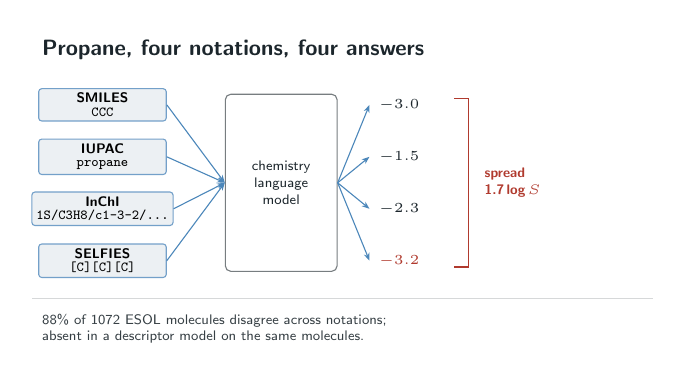
\begin{tikzpicture}[
  x=1cm, y=1cm,
  note/.style={draw=rscblue!55, fill=soft, rounded corners=1.1pt,
               inner sep=1.6pt, minimum width=1.62cm, align=center,
               font=\tiny},
  val/.style={font=\tiny\bfseries, align=left},
  ar/.style={-{Stealth[length=2.8pt]}, rscblue!70, line width=0.4pt},
]

\useasboundingbox (0,0) rectangle (8,4);

% ---- title ----
\node[anchor=north west, font=\footnotesize\bfseries, text=ink]
      at (0.06,3.97) {Propane, four notations, four answers};

% ---- notation inputs ----
\node[note] (a) at (0.95,3.02) {\textbf{SMILES}\\[-1pt]\texttt{CCC}};
\node[note] (b) at (0.95,2.36) {\textbf{IUPAC}\\[-1pt]\texttt{propane}};
\node[note] (c) at (0.95,1.70) {\textbf{InChI}\\[-1pt]\texttt{1S/C3H8/c1-3-2/...}};
\node[note] (d) at (0.95,1.04) {\textbf{SELFIES}\\[-1pt]\texttt{[C][C][C]}};

% ---- model ----
\node[draw=ink!60, fill=white, rounded corners=2pt, minimum width=1.42cm,
      minimum height=2.25cm, align=center, font=\tiny, text=ink]
      (m) at (3.22,2.03) {chemistry\\language\\model};

\foreach \n in {a,b,c,d}{\draw[ar] (\n.east) -- (m.west);}

% ---- diverging predictions ----
\node[val, text=ink]  (p1) at (4.72,3.02) {$-3.0$};
\node[val, text=ink]  (p2) at (4.72,2.36) {$-1.5$};
\node[val, text=ink]  (p3) at (4.72,1.70) {$-2.3$};
\node[val, text=warn] (p4) at (4.72,1.04) {$-3.2$};

\foreach \p in {p1,p2,p3,p4}{\draw[ar] (m.east) -- (\p.west);}

% ---- spread bracket ----
\draw[warn, line width=0.55pt]
      (5.42,3.10) -- (5.60,3.10) -- (5.60,0.96) -- (5.42,0.96);
\node[anchor=west, font=\tiny\bfseries, text=warn, align=left]
      at (5.68,2.03) {spread\\1.7\,log\,$S$};

% ---- footer ----
\draw[ink!18, line width=0.4pt] (0.06,0.56) -- (7.94,0.56);
\node[anchor=north west, font=\tiny, text=ink!88, align=left]
      at (0.06,0.48)
      {88\% of 1072 ESOL molecules disagree across notations;\\[-0.5pt]
       absent in a descriptor model on the same molecules.};

\end{tikzpicture}
\end{document}
